\documentclass[11pt]{article}

% Transcription of the handwritten lecture notes "Lecture-02.pdf"
% (7 pages: Brownian motion + Itô calculus).
\usepackage{amsmath,amssymb,amsthm,mathtools}
\usepackage[margin=1in]{geometry}
\usepackage{xcolor}
\usepackage{tikz}
\usepackage[hidelinks]{hyperref}

% ---- macros -------------------------------------------------------------
\newcommand{\Prob}{\mathbb{P}}
\newcommand{\E}{\mathbb{E}}
\newcommand{\R}{\mathbb{R}}
\newcommand{\F}{\mathcal{F}}
\newcommand{\dd}{\,\mathrm{d}}
\newcommand{\ind}{\mathbf{1}}                 % indicator
\newcommand{\cnum}[1]{\textcircled{\raisebox{-0.6pt}{\scriptsize #1}}} % circled example numbers
\newcommand{\Var}{\operatorname{Var}}
\newcommand{\Cov}{\operatorname{Cov}}

% The notes' blue handwritten annotations are reproduced in blue.
\newcommand{\ann}[1]{\textcolor{blue}{#1}}

\theoremstyle{definition}
\newtheorem{proposition}{Proposition}

\title{\textbf{MFM5210 Stochastics and Partial Differential Equations}\\[4pt]
\large Lecture 2 --- Brownian motion and It\^o calculus}
\author{Wei Qi}
\date{Sept 14, 2026}

\begin{document}
\maketitle

\section{Brownian motion}

A \emph{standard Brownian motion} (BM in short) is a stochastic process
$B=\{B_t\}_{t\ge0}$ with

\begin{enumerate}
\item $B_0=0$;
\item \emph{independent increments}: $\forall n\ge1$, $\forall 0\le t_1<t_2<\cdots<t_n<\infty$,
      $B_{t_2}-B_{t_1}$, $B_{t_3}-B_{t_2}$, $\ldots$, $B_{t_n}-B_{t_{n-1}}$ are independent;
\item \emph{stationary \& normal increments}: $\forall 0\le s<t$, $B_t-B_s\sim N(0,t-s)$;
\item $B_t$ is continuous (as a function of $t$).
\end{enumerate}

\begin{center}
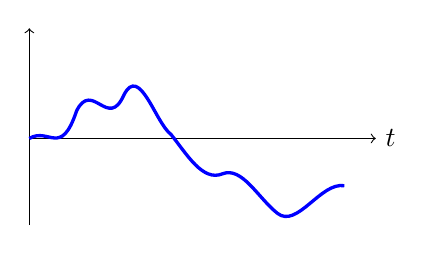
\begin{tikzpicture}[scale=1]
  \draw[->] (0,0) -- (4.4,0) node[right]{$t$};
  \draw[->] (0,-1.1) -- (0,1.4);
  \draw[very thick,blue]
    (0,0) .. controls (0.25,0.15) and (0.4,-0.25) .. (0.6,0.35)
          .. controls (0.8,0.75) and (1.0,0.1) .. (1.2,0.55)
          .. controls (1.4,0.95) and (1.6,0.2) .. (1.8,0.05)
          .. controls (2.0,-0.2) and (2.2,-0.55) .. (2.45,-0.45)
          .. controls (2.7,-0.35) and (2.9,-0.75) .. (3.15,-0.95)
          .. controls (3.4,-1.15) and (3.7,-0.55) .. (4.0,-0.6);
\end{tikzpicture}
\end{center}

\noindent\textbf{Remark.} $B$ is called BM starting from $x$ if (1) is replaced by $B_0=x$.

\medskip
\noindent Recall the definition of \emph{independence}:

\begin{enumerate}
\item[(i)] $A,B\in\F$ are independent if $\Prob(A\cap B)=\Prob(A)\cdot\Prob(B)$.
\item[(ii)] r.v.s $X$, $Y$ are independent if
      $\Prob\{X\le a,\;Y\le b\}=\Prob\{X\le a\}\cdot\Prob\{Y\le b\}$
      $\forall a,b\in\R$.
\item[(iii)] r.v.s $X_1,\ldots,X_n$ are independent if $\forall k=1,\ldots,n$, for any $k$ of them
      $X_{i_1},\ldots,X_{i_k}$ and any $a_1,\ldots,a_k\in\R$,
      \[
        \Prob\{X_{i_1}\le a_1,\;\ldots,\;X_{i_k}\le a_k\}
        =\Prob\{X_{i_1}\le a_1\}\cdots\Prob\{X_{i_k}\le a_k\}.
      \]
\item[(iv)] $X$, $Y$ independent $\Rightarrow$
      \[
        \E[XY]=\E[X]\E[Y],\qquad \E[f(X)g(Y)]=\E[f(X)]\E[g(Y)]
      \]
      provided all expectations exist.
\end{enumerate}

\section{Examples}

\noindent\cnum{1} \textbf{Compute the covariance of BM.} Suppose $0<s<t$. Then
\begin{align*}
  \E[B_sB_t]
    &= \E\bigl[B_s(B_t-B_s+B_s)\bigr]\\
    &= \E\bigl[B_s(B_t-B_s)\bigr]+\E[B_sB_s]\\
    &= \underbrace{\E[B_s]}_{=0}\cdot\underbrace{\E[B_t-B_s]}_{=0}+\underbrace{\E[B_s^2]}_{=\Var(B_s)=s}
       \qquad\text{(independence)}\\
    &= s .
\end{align*}
\ann{(Side note: $B_s-B_0\sim N(0,s-0)$, hence $B_s\sim N(0,s)$.)}

\smallskip
\noindent Conclusion: $\Cov(B_s,B_t)=\E[B_sB_t]=\min\{s,t\}$
\ann{(also denoted by $s\wedge t$)}.

\medskip
\noindent\cnum{2} \textbf{Compute the $n$-th moment $\E[B_t^n]$, where $n\ge1$ is an integer.}

\begin{itemize}
\item Recall: if $X$ has density $f(x)$, then
      $\E[\varphi(X)]=\displaystyle\int_{-\infty}^{\infty}\varphi(x)f(x)\dd x$.
      Since $B_t\sim N(0,t)$, $B_t$ has density
      $f_t(x)=\dfrac{1}{\sqrt{2\pi t}}e^{-x^2/(2t)}$.
\item By a change of variable ($x=\sqrt{t}\,y$):
      \[
        \E[B_t^n]=\frac{1}{\sqrt{2\pi t}}\int_{-\infty}^{\infty}x^ne^{-x^2/(2t)}\dd x
        =t^{n/2}\cdot\frac{1}{\sqrt{2\pi}}\int_{-\infty}^{\infty}y^ne^{-y^2/2}\dd y
        =t^{n/2}\;\underbrace{\E[Z^n]}_{Z\sim N(0,1)} .
      \]
\item If $n$ is odd, then $y^ne^{-y^2/2}$ is an odd function, so $\E[Z^n]=0$.
\item If $n$ is even, it follows from integration by parts that
      \begin{align*}
        \E[Z^n]
          &= -\frac{1}{\sqrt{2\pi}}\int_{-\infty}^{\infty}y^{n-1}\dd\bigl(e^{-y^2/2}\bigr)\\
          &= -\frac{1}{\sqrt{2\pi}}
             \Bigl[\underbrace{y^{n-1}e^{-y^2/2}\Big|_{-\infty}^{\infty}}_{=0}
             -\int_{-\infty}^{\infty}(n-1)y^{n-2}e^{-y^2/2}\dd y\Bigr]\\
          &= (n-1)\,\frac{1}{\sqrt{2\pi}}\int_{-\infty}^{\infty}y^{n-2}e^{-y^2/2}\dd y\\
          &= (n-1)\,\E[Z^{n-2}]\\
          &= (n-1)(n-3)\,\E[Z^{n-4}]\\
          &= (n-1)(n-3)\cdots3\cdot\underbrace{1}_{\E[Z^2]=1}
             \qquad\text{(by induction).}
      \end{align*}
\end{itemize}

\noindent Conclusion:
\[
  \E[B_t^n]=
  \begin{cases}
    0, & \text{if $n$ is odd},\\[4pt]
    (n-1)(n-3)\cdots3\cdot1\cdot t^{n/2}, & \text{if $n$ is even}.
  \end{cases}
\]
e.g.\ $\E[B_t^2]=t$, \; $\E[B_t^4]=3t^2$, \; $\E[B_t^6]=15t^3$.

\medskip
\noindent\cnum{3} \textbf{Compute $\E[B_1^2B_3^2]$.}
\begin{align*}
  \E[B_1^2B_3^2]
    &= \E\bigl[B_1^2(B_3-B_1+B_1)^2\bigr]\\
    &= \underbrace{\E\bigl[B_1^2(B_3-B_1)^2\bigr]}_{\text{independent}}
       +\underbrace{\E[B_1^4]}_{=3}
       +2\underbrace{\E\bigl[B_1^3(B_3-B_1)\bigr]}_{\text{independent}}\\
    &= \E[B_1^2]\,\E[(B_3-B_1)^2]+3+2\underbrace{\E[B_1^3]}_{=0}\cdot\underbrace{\E[B_3-B_1]}_{=0}\\
    &= 1\cdot2+3+0=5 .
\end{align*}

\medskip
\noindent\cnum{4} \textbf{Compute the moment generating function $\E[e^{aB_t}]$, $a\in\R$.}
\begin{align*}
  \E[e^{aB_t}]
    &= \frac{1}{\sqrt{2\pi t}}\int_{-\infty}^{\infty}e^{ax}e^{-x^2/(2t)}\dd x\\
    &= \frac{1}{\sqrt{2\pi t}}\int_{-\infty}^{\infty}
       e^{-\frac{1}{2t}\left(x^2-2atx+a^2t^2\right)}\,e^{a^2t/2}\dd x\\
    &= e^{a^2t/2}\cdot\frac{1}{\sqrt{2\pi t}}\int_{-\infty}^{\infty}
       e^{-(x-at)^2/(2t)}\dd x
       \qquad \ann{\text{($=1$: pdf of $N(at,t)$)}}
\end{align*}
\noindent Conclusion: $\E[e^{aB_t}]=e^{a^2t/2}$ \quad $\forall a\in\R$, $\forall t\ge0$.

\section{It\^o calculus}

Let $\{B_t\}_{t\ge0}$ be a standard BM and $\F_t=\F_t^B$ be its natural filtration. Fix $T>0$.
For certain processes $\{f_t\}_{t\in[0,T]}$, we define the \emph{It\^o integral}
\[
  \int_0^Tf_t\dd B_t
  \qquad\Bigl(\text{or }\int_0^Tf(t,\omega)\dd B_t\Bigr).
\]
We briefly describe the construction and some basic properties.

\subsection*{Construction of $\int_0^Tf_t\dd B_t$ \ \ann{(or elementary)}}

\noindent\textbf{Step 1.} Suppose $f_t=\varphi(t,\omega)$ is a \emph{simple predictable process}
of the form
\[
  \varphi_t=\varphi(t,\omega)=\sum_{j=1}^na_j(\omega)\,\ind_{t_{j-1}<t\le t_j}
\]
for some $0=t_0<t_1<\cdots<t_n=T$ and r.v.s $a_1,\ldots,a_n$, where
``predictable'' means every $a_j$ is $\F_{t_{j-1}}$-measurable
($a_j\in\F_{t_{j-1}}$). Define
\[
  \int_0^T\varphi_t\dd B_t=\sum_{j=1}^na_j\bigl(B_{t_j}-B_{t_{j-1}}\bigr).
\]

\smallskip
\noindent\textbf{Example.}
\[
  \varphi_t=2\cdot\ind_{0<t\le1}+5B_1\cdot\ind_{1<t\le3}+B_1B_3\cdot\ind_{3<t\le4},
  \qquad t\in[0,4].
\]
$\varphi$ is predictable since
\ann{$a_1=2\in\F_0$ (the only $\F_0$-measurable r.v.s are constants)}, \;
$a_2=5B_1\in\F_1$, \;
$a_3=B_1B_3\in\F_3$.

\begin{center}
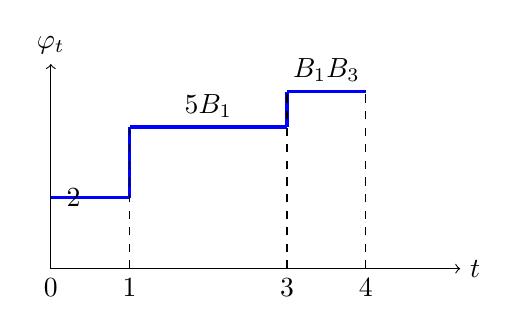
\begin{tikzpicture}[scale=1]
  \draw[->] (0,0) -- (5.2,0) node[right]{$t$};
  \draw[->] (0,0) -- (0,2.6) node[above]{$\varphi_t$};
  \draw[very thick,blue] (0,0.9) -- (1,0.9);
  \draw[very thick,blue] (1,0.9) -- (1,1.8);
  \draw[very thick,blue] (1,1.8) -- (3,1.8);
  \draw[very thick,blue] (3,1.8) -- (3,2.25);
  \draw[very thick,blue] (3,2.25) -- (4,2.25);
  \draw[dashed] (1,0) -- (1,1.8);
  \draw[dashed] (3,0) -- (3,2.25);
  \draw[dashed] (4,0) -- (4,2.25);
  \node[below] at (0,0) {$0$};
  \node[below] at (1,0) {$1$};
  \node[below] at (3,0) {$3$};
  \node[below] at (4,0) {$4$};
  \node[left] at (0.5,0.9) {$2$};
  \node[above] at (2,1.8) {$5B_1$};
  \node[above] at (3.5,2.25) {$B_1B_3$};
\end{tikzpicture}
\end{center}

\[
  \int_0^4\varphi_t\dd B_t=2(B_1-B_0)+5B_1(B_3-B_1)+B_1B_3(B_4-B_3).
\]

\medskip
\noindent\textbf{Step 2.} \ann{Following \O ksendal's notation:} suppose
$g=\{g_t\}_{t\in[0,T]}\in V(0,T)$, which means:
\begin{enumerate}
\item[(0)] $g(t,\omega)$ is $\mathcal{B}(\R)\otimes\F$-measurable
      (a technical assumption satisfied by all simple processes and all piecewise
      continuous processes; we take it for granted for all processes in this course);
\item[(1)] $\{g_t\}_{t\in[0,T]}$ is adapted to $\{\F_t\}_{t\in[0,T]}$; and
\item[(2)] $\E\bigl[\int_0^T|g(t,\omega)|^2\dd t\bigr]<\infty$.
\end{enumerate}
For $g\in V(0,T)$, we define $\int_0^Tg_t\dd B_t$ via the following approximation
procedure: \ann{(see \O ksendal for details)}

\smallskip
\noindent\textbf{Fact.} For any $\{g(t,\omega)\}_{t\in[0,T]}\in V(0,T)$, we can find a sequence
$\varphi_n=\{\varphi_n(t,\omega)\}_{t\in[0,T]}$ of simple predictable processes such that
``\ann{$\varphi_n\to g$ as $n\to\infty$ in a suitable sense}''.
For each $n$, the It\^o integral $\int_0^T\varphi_n(t,\omega)\dd B_t$ has been defined,
thanks to Step 1. Finally, it can be shown that the r.v.s
$\int_0^T\varphi_n(t,\omega)\dd B_t$ have a limit (as $n\to\infty$), which is therefore
defined as
\[
  \int_0^Tg_t\dd B_t \qquad\text{or}\qquad \int_0^Tg(t,\omega)\dd B_t .
\]
For any $0\le a\le b\le T$, define
\[
  \int_a^bg_t\dd B_t=\int_0^bg_t\dd B_t-\int_0^ag_t\dd B_t .
\]

\begin{proposition}[Properties of It\^o integrals]
Let $f,g\in V(0,T)$.
\begin{enumerate}
\item[(i)] \ann{(Linearity)} $\forall$ constants $c_1,c_2\in\R$,
      \[
        \int_0^T(c_1f_t+c_2g_t)\dd B_t
        =c_1\int_0^Tf_t\dd B_t+c_2\int_0^Tg_t\dd B_t .
      \]
\item[(ii)] $\E\bigl[\int_0^Tg_t\dd B_t\bigr]=0$.
\item[(iii)] \ann{(It\^o isometry)}
      $\E\bigl[\bigl(\int_0^Tg_t\dd B_t\bigr)^2\bigr]
       =\E\bigl[\int_0^T|g_t|^2\dd t\bigr]$. \hfill$(\ast)$
\item[(iv)] Let $X_t=\int_0^tg_s\dd B_s$. Then the process $\{X_t\}_{t\in[0,T]}$ is
      continuous \ann{almost surely} and is $\F_t$-adapted.
      \ann{(a.s.\ = with prob.\ 1)}
\end{enumerate}
\end{proposition}

\noindent Recall that $\F_t=\F_t^B$ is the natural filtration of $\{B_t\}$. \;
(Proofs omitted; see \O ksendal Ch.~3.)

\medskip
\noindent\textbf{Remark.} Thanks to Fubini's theorem, we may further compute $(\ast)$ by
\[
  \E\Bigl[\int_0^T|g_t|^2\dd t\Bigr]=\int_0^T\E\bigl[|g_t|^2\bigr]\dd t .
\]

\subsection*{Examples}

\noindent\cnum{1} $g_t\equiv1$. Then $g_t\in V(0,T)$, since
\[
  \begin{cases}
    1\in\F_0\subset\F_t \quad \forall t,\\[2pt]
    \E\bigl[\int_0^T1^2\dd t\bigr]=T<\infty .
  \end{cases}
\]
Hence
\[
  \int_0^Tg_t\dd B_t=\int_0^T1\dd B_t=1\cdot(B_T-B_0)=B_T
  \qquad \ann{\text{(by Step 1, for a simple process)}}
\]
\begin{center}
\begin{tikzpicture}[scale=0.9]
  \draw[->] (0,0) -- (4.2,0) node[right]{$T$};
  \draw[->] (0,0) -- (0,1.6);
  \draw[very thick,blue] (0,1) -- (3.4,1);
  \node[left] at (0,1) {$1$};
  \node[below left] at (0,0) {$0$};
\end{tikzpicture}
\end{center}

\medskip
\noindent\cnum{2} Simple predictable processes belong to $V(0,T)$ provided
$\E[a_j^2]<\infty$, e.g.\ the $\varphi_t$ above. Then $\int_0^4\varphi_t\dd B_t$ is a r.v.
with mean $0$ (but not normally distributed). Its variance can be computed using
It\^o's isometry:
\begin{align*}
  \E\Bigl[\Bigl(\int_0^4\varphi_t\dd B_t\Bigr)^2\Bigr]
    &= \E\Bigl[\int_0^4\varphi_t^2\dd t\Bigr]
     = \int_0^4\E[\varphi_t^2]\dd t\\
    &= \E[2^2]\,(1-0)+\E[25B_1^2]\,(3-1)+\E[B_1^2B_3^2]\,(4-3)\\
    &= 4+50+5=59 .
\end{align*}

\medskip
\noindent\cnum{3} $\{B_t\}_{t\in[0,T]}\in V(0,T)$:
\begin{itemize}
\item $B_t\in\F_t$ for each $t\in[0,T]$ \ann{(by definition of $\F_t^B$)};
\item $\E\bigl[\int_0^T|B_t|^2\dd t\bigr]=\int_0^T\E[B_t^2]\dd t=\int_0^Tt\dd t
      =\dfrac{T^2}{2}<\infty$ \ann{(as $\E[B_t^2]=t$)}.
\end{itemize}
Hence $\int_0^TB_t\dd B_t$ is well defined. It is a r.v.\ with mean $0$ and variance
\[
  \E\Bigl[\Bigl(\int_0^TB_t\dd B_t\Bigr)^2\Bigr]=\int_0^T\E[B_t^2]\dd t=\frac{T^2}{2} .
\]

\medskip
\noindent\textbf{Exercise.} Verify that $\{B_t^2\}_{t\in[0,T]}\in V(0,T)$ and compute the
variance of $\int_0^TB_t^2\dd B_t$.

\medskip
\noindent\textbf{Question.} How to compute/simplify $\int_0^Tg_t\dd B_t$ in general?
This can be done using \emph{It\^o's formula}, a central tool of It\^o calculus.

\end{document}
